%%% template.tex
%%%
%%% This LaTeX source document can be used as the basis for your technical
%%% paper or abstract. Intentionally stripped of annotation, the parameters
%%% and commands should be adjusted for your particular paper - title, 
%%% author, article DOI, etc.
%%% The accompanying ``template.annotated.tex'' provides copious annotation
%%% for the commands and parameters found in the source document. (The code
%%% is identical in ``template.tex'' and ``template.annotated.tex.'')

\documentclass[conference, 12pt]{acmsiggraph}

\title{Reconstructing scenes from photos using Global SfM}

\author{Bryce Evans \and Rafael Farias Marinheiro}
% \contactemail{}
\affiliation{Cornell University\thanks{\{bae43, rf356\}@cornell.edu}}
\pdfauthor{Rafael F. Marinheiro}

\keywords{crowd simulation, user interaction, real-time rendering}

\usepackage{amsmath}


\begin{document}

%% \teaser{
%%   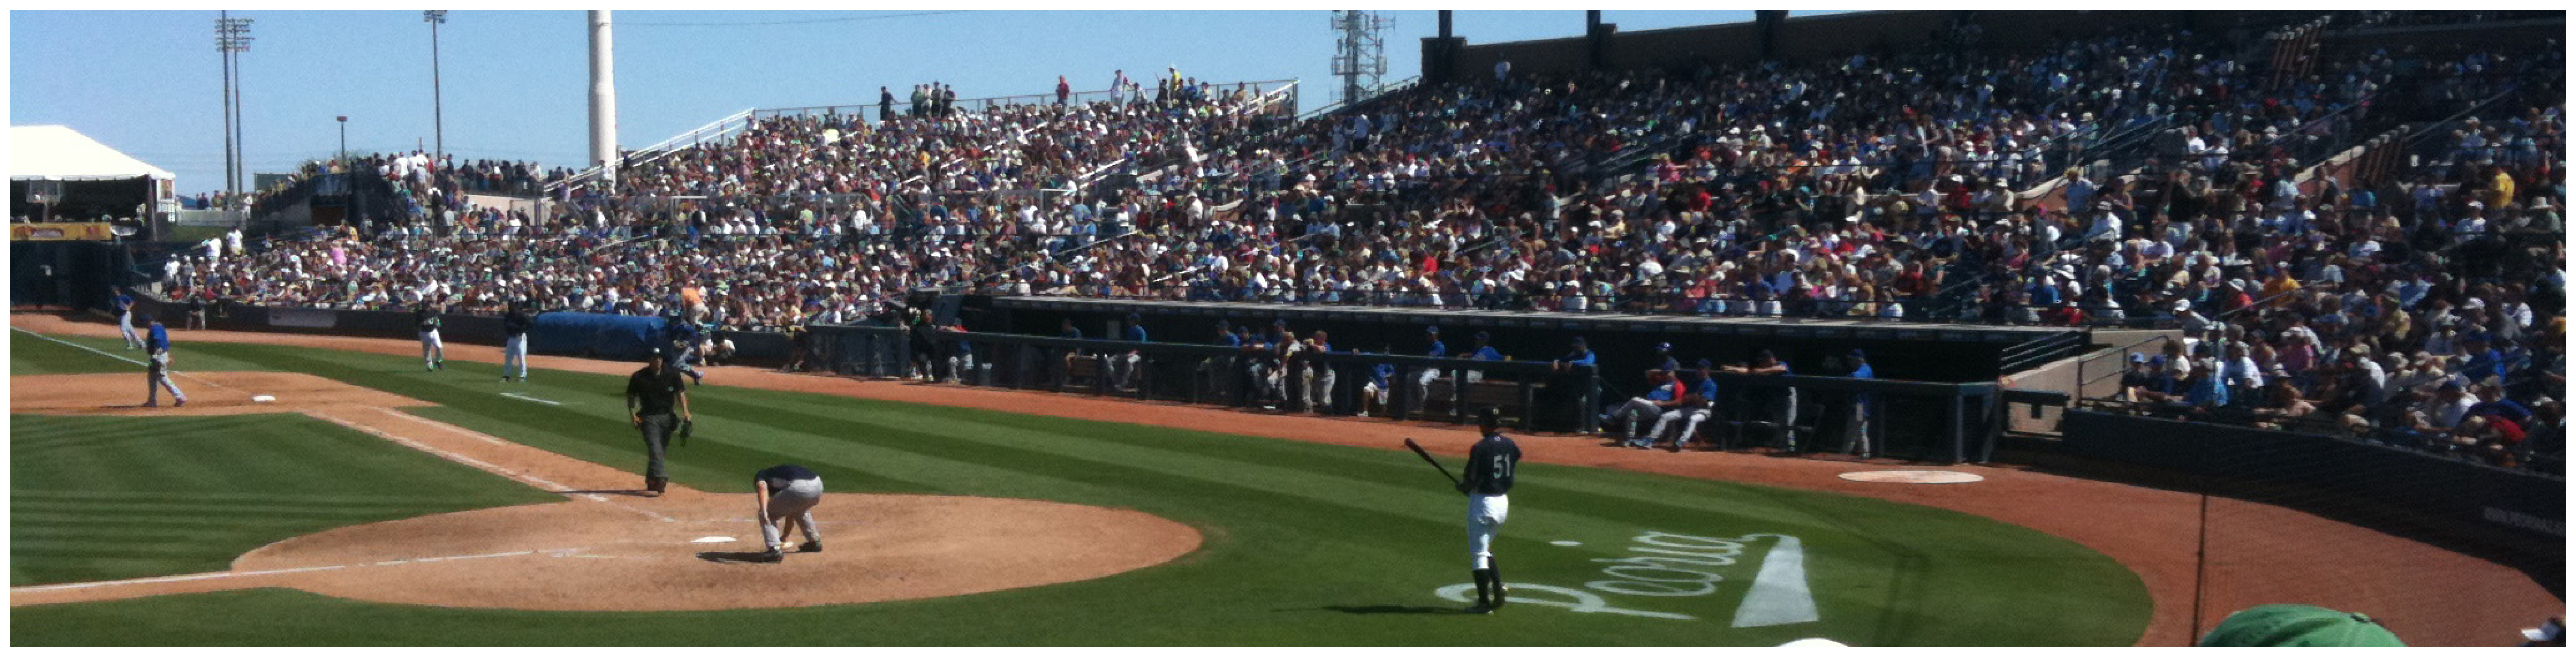
\includegraphics[height=1.5in]{images/sampleteaser}
%%   \caption{Spring Training 2009, Peoria, AZ.}
%% }

\maketitle

% \begin{abstract}

% We intend to create a interactive Crowd Simulation application using the approach described in \cite{kim2012interactive}. The user will be able to interact with the application with a commodity depth sensor \cite{Zhang:2012:MKS:2225053.2225203}, modifying the environment in real time.

% \end{abstract}

% \begin{figure}[Ht!]
%   \centering
%     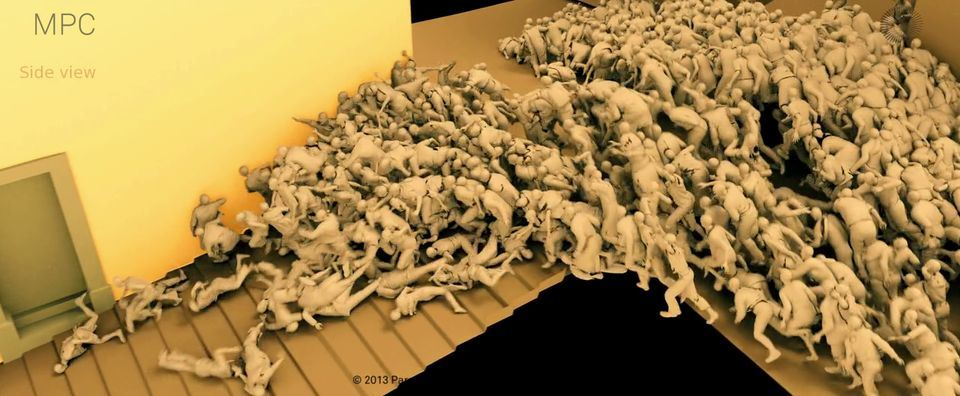
\includegraphics[width=0.5\textwidth]{images/mpc3.jpg}
%     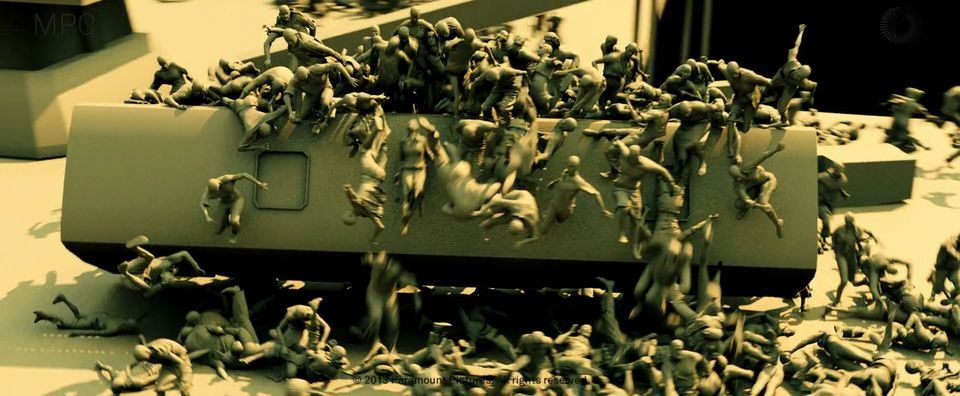
\includegraphics[width=0.5\textwidth]{images/mpc2.jpg}
% 	\caption{World War Z (2013). Zombie agents were computationally simulated.}
% 	\label{fig:wwz}
% \end{figure}

% %% Use this only if you're preparing a technical paper to be published in the 
% %% ACM 'Transactions on Graphics' journal.

% \begin{CRcatlist}
% 	\CRcat{I.2.11}{Artificial Intelligence}{Distributed Artificial Intelligence}{Multiagent systems};
% 	\CRcat{I.3.7}{Computer Graphics}{Three-Dimensional Graphics and Realism}{Animation};
% 	\CRcat{I.6.8}{Simulation and Modeling}{Types of Simulation}{Animation}
% \end{CRcatlist}

% %%% The ``\keywordlist'' prints out the user-defined keywords.

% \keywordlist

% \TOGlinkslist

% %% Required for all content. 

% \copyrightspace

\section{Problem}

Large image sets are around us everyday but give little understanding into the scenes they are of. Making use of data to create 3D geometry could give strong representations of buildings for navigating cities or reconstructing objects to save modeling time. Applications such as Google Maps make use of these large image sets to reconstruct landscapes, but making a system more robust for disorganized sets and generalized to generating a 3D mesh for any geometry would have greater application.


\section{Goals}

We intend to implement a Global Structure from Motion technique to reconstruct scenes from photos. We will use the techniques described by \cite{rotation} and \cite{translation}. If we run into time constraints, we will use the code for \cite{rotation} (which is available online) and we will implement the translation correction ourselves. We intend to use our implementation with a large dataset obtained from the internet.

\section{Schedule}

Plan A:

\begin{itemize}
	\item {Week of October 13th}: Project Proposal Presentation
	\item {Week of October 20th}: Feature Detection and Feature Matching
	\item {Week of October 27th}: Homography Computation and Relative Rotation/Translation computation
	\item {Week of November 3rd}: Homography Computation and Relative Rotation/Translation computation
	\item {Week of November 10th}: Rotation Averaging
	\item {Week of November 17th}: Rotation Averaging
	\item {Week of November 24th}: Translation Correction
	\item {Week of November 1st}: Translation Correction
	\item {Week of November 8th}:


\end{itemize}



\bibliographystyle{acmsiggraph}
\bibliography{proposal}
\end{document}
